\documentclass[a4paper, 11pt]{article}

% --- PREAMBLE ---
\usepackage[utf8]{inputenc}
\usepackage[T1]{fontenc}
\usepackage[a4paper, margin=2.5cm]{geometry} % Set A4 paper size and margins
\usepackage{graphicx}
\usepackage{amsmath}
\usepackage{booktabs}
\usepackage{fancyvrb} % For Verbatim
\usepackage{fvextra} % For breaklines in Verbatim (Note: Removed breaklines option below due to errors)
\usepackage[hidelinks]{hyperref}
\usepackage{tikz}
\usetikzlibrary{er, positioning, arrows.meta}
% \usepackage{lipsum} % Removed placeholder text package
\usepackage{float} % For [H] figure placement
\usepackage{url} % For formatting URLs

% --- TIKZ ERD STYLES ---
\tikzstyle{entity} = [
    rectangle, draw, thick,
    minimum width=3.5cm, minimum height=1.2cm, % Adjusted size slightly
    text width=3.3cm, text centered, align=left % Align text left within nodes
]
\tikzstyle{weak entity} = [
    entity, double,
]
\tikzstyle{attribute} = [
    ellipse, draw, thick,
    minimum width=3cm, minimum height=1cm,
    text width=2.8cm, text centered
]
\tikzstyle{key attribute} = [
    attribute,
    font=\underline
]
\tikzstyle{relationship} = [
    diamond, draw, thick,
    minimum width=3cm, minimum height=1.2cm, % Adjusted size slightly
    text width=2.8cm, text centered
]
\tikzstyle{weak relationship} = [
    relationship, double,
]
\tikzstyle{isa} = [
    isosceles triangle, draw, thick,
    minimum width=2cm, minimum height=1.5cm,
    shape border rotate=90, text centered
]

% --- DOCUMENT START ---
\begin{document}

\title{TuneTrace: Design and Implementation of a Database System for a Hybrid Music Recommendation Service}

\author{
    Agrannya Singh \\
    \textit{School Of Computer Science And Engineering } \\
    \textit{Vellore Institute of Technology , Vellore}\\
    23BCE0965 \\
    \texttt{singh.agrannya@gmail.com}
}

\date{\today} % Use today's date
\maketitle

% --- ABSTRACT ---
\begin{abstract}
This report details the database management system architecture and implementation for TuneTrace, a FastAPI microservice designed to provide hybrid music recommendations. The system's core function is to analyze a user's liked songs and generate personalized suggestions primarily through database-driven collaborative filtering. This necessitates a robust database backend to persist user profiles, song metadata, and the many-to-many relationships between them. This project leverages a PostgreSQL relational database managed via the SQLAlchemy Object Relational Mapper (ORM), with SQLite as a development fallback. Key database features include a normalized schema design, a data access layer implemented using the repository pattern, complex SQL generation via the ORM for the recommendation algorithm, a multi-layer caching strategy involving Redis and in-memory LRU caches for performance optimization, and schema evolution management with Alembic. This paper explores the conceptual, logical, and physical design of the database, the implementation details of data operations based on the provided Python codebase, transaction management, indexing strategies, and proposed schema extensions using Extended Entity-Relationship (EER) modeling concepts to support future features.
\end{abstract}

% --- KEYWORDS ---
\begin{center}
\textbf{Keywords}
\end{center}
\small
Database Management Systems, DBMS, PostgreSQL, SQLAlchemy, ER Modeling, EER, Collaborative Filtering, FastAPI, Alembic, Caching, Redis, ORM, Data Modeling, Schema Evolution, Performance Optimization.
\normalsize
\vspace{1em}


% --- I. INTRODUCTION ---
\section{Introduction}
The proliferation of digital music platforms has created an immense need for effective recommendation systems that can help users navigate vast catalogs and discover new content aligned with their tastes. The TuneTrace project addresses this need by providing a backend microservice designed to deliver high-quality, personalized song recommendations. Built using the Python FastAPI framework, the service exposes a RESTful API allowing client applications (such as web or mobile apps) to submit a user's liked songs and receive a curated list of new suggestions derived primarily from YouTube music content.

The core challenge in building such a system lies in efficiently managing the data representing users, songs, and their interactions. A robust Database Management System (DBMS) is fundamental to the service's operation. Its key responsibilities include:
\begin{enumerate}
    \item \textbf{User Profile Persistence:} Securely storing user information, enabling identification through unique identifiers, typically derived from an OAuth provider like Google (e.g., user email address).
    \item \textbf{Song Catalog Management:} Maintaining a canonical catalog of song metadata. This involves retrieving data from external sources, such as the YouTube Data API, and storing relevant attributes like title, artist (channel), and potentially genre or tags, ensuring uniqueness based on the external identifier (YouTube Video ID).
    \item \textbf{Interaction Tracking:} Recording the relationship between users and the songs they express a preference for (e.g., "likes"). This inherently represents a many-to-many relationship, as one user can like multiple songs, and one song can be liked by many users.
    \item \textbf{Complex Query Execution:} Supporting the execution of sophisticated queries required by the recommendation algorithm. Specifically, the collaborative filtering approach implemented in TuneTrace requires identifying users with similar taste profiles based on overlapping liked songs and then suggesting songs liked by those similar users.
\end{enumerate}

This report provides a comprehensive analysis of the database system designed and implemented for the TuneTrace backend, based on the provided codebase and documentation (including \texttt{main.py}, \texttt{db.py}, Alembic migrations, and various markdown files). It details the journey from conceptual data modeling to the physical implementation using PostgreSQL (with SQLite as a fallback) and the SQLAlchemy Object Relational Mapper (ORM). Key areas covered include the logical schema design represented via Entity-Relationship (ER) diagrams, the implementation of data manipulation operations within the repository pattern, strategies employed for performance optimization such as indexing and multi-layer caching (Redis and LRU), and the management of schema changes over time using Alembic. Furthermore, the report explores potential future enhancements to the schema using Extended Entity-Relationship (EER) concepts, demonstrating a forward-looking approach to the system's data architecture. This document aims to illustrate the practical application of database principles in developing a functional and scalable recommendation microservice.

% --- II. RELATED WORK ---
\section{Related Work}
Recommendation systems represent a significant field within data management, information retrieval, and machine learning, aiming to predict user preferences for items \cite{1}. The design of the underlying database system is heavily influenced by the chosen recommendation strategy. The two foundational approaches are content-based filtering and collaborative filtering (CF), with hybrid systems often combining elements of both.

\subsection{Content-Based Filtering}
Content-based recommendation systems operate by identifying items with attributes similar to those the user has positively interacted with in the past. For a music recommendation system like TuneTrace, this would involve analyzing metadata associated with songs, such as genre, artist, album, tempo, instrumentation, or even lyrical content. The system would build a profile of the user's preferences based on the attributes of the songs they like and then recommend other songs sharing those attributes.

Implementing a content-based system heavily relies on a well-structured database containing detailed item metadata. This often leads to a highly normalized schema. For instance, separate tables might exist for \texttt{Artists}, \texttt{Albums}, \texttt{Genres}, and \texttt{Songs}, with relationships defined between them (e.g., a song belongs to an album, an album is by an artist, a song has one or more genres). Recommendation generation involves querying this schema to find songs whose attribute vectors are close (e.g., using cosine similarity) to the user's preference profile vector. While effective in recommending variations of known preferences, content-based systems can suffer from limited serendipity (difficulty recommending items outside the user's established taste profile) and require extensive, high-quality metadata for all items. The initial TuneTrace schema partially supports this by storing a \texttt{genre} field, which is used in its fallback mechanism.

\subsection{Collaborative Filtering (CF)}
Collaborative filtering techniques, in contrast, leverage the collective behavior of users – the "wisdom of the crowd" – to make recommendations \cite{2}. They operate under the assumption that users who agreed in the past (e.g., liked the same songs) will likely agree in the future. CF methods do not require knowledge about the items' attributes; they rely solely on the user-item interaction matrix (e.g., likes, ratings, purchases).

There are two primary categories of CF:
\begin{itemize}
    \item \textbf{User-Based CF:} This approach identifies users whose past interactions (likes) are similar to the active user's interactions. Recommendations are then generated from items that these "neighboring" or "similar" users have liked but the active user has not yet encountered. The core database operation involves finding users with significant overlap in liked items.
    \item \textbf{Item-Based CF:} This method calculates similarities between items based on how users have interacted with them. For example, if many users who liked Song A also liked Song B, the system infers that Song A and Song B are similar. Recommendations for an active user are then generated by finding items similar to those the user has already liked. This often involves pre-computing an item-item similarity matrix.
\end{itemize}

The TuneTrace service, as implemented in \texttt{main.py} within the \texttt{MusicRepository.get\_collaborative\_suggestions} method, explicitly employs a **user-based collaborative filtering** strategy. The database is central to this approach, as the algorithm directly queries the \texttt{user\_liked\_songs} table (representing the interaction matrix) to find similar users based on shared liked \texttt{song\_id}s and then aggregates suggestions from those users. This database-centric implementation contrasts with model-based CF approaches (like matrix factorization) that learn latent factors from the interaction data.

\subsection{Hybrid Approaches}
Many modern recommendation systems employ hybrid strategies that combine CF and content-based methods to leverage their respective strengths and mitigate weaknesses. For example, CF can struggle with the "cold start" problem (making recommendations for new users or new items with no interaction history), where content-based methods might still function if metadata is available. TuneTrace implements a simple hybrid model: it prioritizes the user-based CF algorithm. However, if this algorithm fails to produce sufficient suggestions (e.g., for a new user or a user with unique tastes yielding no similar neighbors meeting the criteria), it falls back to a content-based approach by calling \texttt{\_get\_fallback\_suggestions}, which retrieves popular songs based on an optional user-provided genre or global top hits directly from the YouTube API.

% --- III. SYSTEM ARCHITECTURE ---
\section{System Architecture}
The TuneTrace backend is designed as a layered microservice, promoting modularity and separation of concerns. This architecture is evident in the structure of the provided codebase, particularly \texttt{main.py} and \texttt{db.py}. The system components interact to handle client requests, process data, and generate recommendations. The production deployment leverages managed services from Render, as indicated in \texttt{render\_configurations.md} and \texttt{DEPLOYMENT.md}.

The key layers and components are:

\begin{enumerate}
    \item \textbf{API Gateway (FastAPI Framework)}: This is the outermost layer, responsible for handling incoming HTTP requests and sending responses. As defined in \texttt{main.py}, FastAPI manages URL routing (e.g., \texttt{@app.post("/suggestions")}), request parsing, and input validation using Pydantic models (e.g., \texttt{LikedSongsRequest}). It also handles response serialization (e.g., returning data conforming to \texttt{SuggestionResponse}). CORS (Cross-Origin Resource Sharing) middleware is configured to allow requests from frontend applications hosted on different domains. FastAPI's dependency injection system is used extensively to provide components like database sessions and service instances to the endpoint functions.

    \item \textbf{Business Logic (Service Layer)}: Encapsulated within the \texttt{SuggestionService} class in \texttt{main.py}. This layer contains the core application logic, orchestrating the recommendation process. It coordinates interactions between the data access layer (repository), external APIs (YouTube), and caching mechanisms. Responsibilities include resolving song names to video IDs, triggering the appropriate recommendation algorithm (collaborative or fallback), and managing the LRU cache for external API calls.

    \item \textbf{Data Access Layer (Repository Pattern)}: Implemented as the \texttt{MusicRepository} class in \texttt{main.py}. This layer abstracts all direct interactions with the database. It utilizes the SQLAlchemy ORM to perform CRUD (Create, Read, Update, Delete) operations on the database entities (\texttt{User}, \texttt{SongMetadata}, \texttt{UserLikedSong}). Key methods include \texttt{get\_or\_create\_user}, \texttt{persist\_user\_likes}, \texttt{get\_user\_liked\_songs}, and the complex \texttt{get\_collaborative\_suggestions} query. This pattern decouples the business logic from the specific database implementation details.

    \item \textbf{Database Session Management}: Defined in \texttt{db.py}. This component configures the connection to the underlying database (PostgreSQL preferred, SQLite fallback) using SQLAlchemy's \texttt{create\_engine}. It provides a session factory (\texttt{SessionLocal}) to create individual database sessions. The \texttt{get\_session} function acts as a FastAPI dependency, ensuring that each incoming API request receives its own isolated database session, which is properly closed after the request is processed. This manages the scope and lifecycle of database transactions.

    \item \textbf{Database (PostgreSQL / SQLite)}: The persistent storage layer. As configured in \texttt{db.py} and mentioned in \texttt{render\_configurations.md}, PostgreSQL is the preferred production database, chosen for its robustness, ACID compliance, and support for complex queries and indexing needed for collaborative filtering. The connection details are sourced from the \texttt{POSTGRES\_DATABASE\_URL} environment variable. A local SQLite database (\texttt{sqlite:///./app.db}) serves as a fallback for development or environments where PostgreSQL is unavailable. SQLAlchemy ORM models in \texttt{db.py} map Python classes to database tables.

    \item \textbf{Caching Subsystem (Redis / In-Memory)}: A multi-layer caching strategy is implemented to enhance performance and reduce load on the database and external APIs.
        \begin{itemize}
            \item \textbf{Redis Cache:} An optional distributed cache (configured via \texttt{REDIS\_URL}) used primarily to store user liked songs (\texttt{user\_likes:\{user\_id\}} key). Updates are performed asynchronously via FastAPI \texttt{BackgroundTasks} (\texttt{update\_redis\_user\_likes} function in \texttt{main.py}) to avoid blocking the API response. It uses a configurable TTL (\texttt{REDIS\_TTL\_SECONDS}).
            \item \textbf{In-Memory LRU Cache:} Python's \texttt{@lru\_cache(maxsize=512)} decorator is applied to the \texttt{\_search\_youtube\_for\_song} method in \texttt{SuggestionService}. This caches results from the YouTube Search API within the application's memory, reducing redundant external calls and mitigating quota usage.
        \end{itemize}

    \item \textbf{External API Integration (YouTube Data API v3)}: The \texttt{SuggestionService} interacts with the YouTube Data API v3, requiring a \texttt{YOUTUBE\_API\_KEY}. It uses the Search endpoint (\texttt{/youtube/v3/search}) to resolve song names to video IDs and metadata (\texttt{\_search\_youtube\_for\_song}) and potentially to fetch popular videos for the fallback mechanism (\texttt{\_get\_fallback\_suggestions}). Error handling and timeouts are implemented for resilience. 
\end{enumerate}

This layered architecture ensures that components are loosely coupled, making the system easier to maintain, test, and scale. The clear separation between API handling, business logic, data access, and external integrations follows standard microservice design principles.

% --- IV. DATABASE DESIGN ---
\section{Database Design and Logical Schema}
The design of the TuneTrace database follows established relational database principles, aiming for data integrity, query efficiency, and scalability. The process involves defining the conceptual model, translating it into a logical schema using ER diagrams, and finally implementing the physical schema using SQLAlchemy ORM models mapped to PostgreSQL/SQLite tables.

\subsection{Conceptual Model}
At the highest level, the core concepts within the TuneTrace domain are:
\begin{itemize}
    \item \textbf{User}: An individual using the service, uniquely identified (e.g., by email).
    \item \textbf{Song}: A piece of music content, uniquely identified (e.g., by YouTube Video ID). A song has metadata like title and artist.
    \item \textbf{Likes Relationship}: Represents a user expressing a preference for a song.
\end{itemize}
The fundamental relationship is between User and Song via the "Likes" interaction. Analyzing the cardinality reveals that a single User can like multiple Songs, and a single Song can be liked by multiple Users. This constitutes a **many-to-many (M:N)** relationship between User and Song. Standard relational database design dictates that M:N relationships cannot be directly implemented; they must be resolved using an intermediary construct.

\subsection{Logical Model (Entity-Relationship Diagram)}
The logical model refines the conceptual model into specific entities, attributes, and relationships suitable for implementation in a relational database. To handle the M:N "Likes" relationship, an **associative entity** (also known as a junction or bridge table) is introduced. In the TuneTrace schema, this is the \texttt{UserLikedSong} entity.

The resulting logical schema consists of three main entities:
\begin{enumerate}
    \item \textbf{User (\texttt{users})}: Represents users. Attributes include a unique internal ID (\texttt{id}), a unique external identifier (\texttt{user\_id}, typically the OAuth email), optional name and email fields, and timestamps (\texttt{created\_at}, \texttt{updated\_at}).
    \item \textbf{SongMetadata (\texttt{song\_metadata})}: Represents songs. Attributes include a unique internal ID (\texttt{id}), the unique YouTube video ID (\texttt{video\_id}), title, artist (channel name), optional genre and tags, and a timestamp (\texttt{updated\_at}).
    \item \textbf{UserLikedSong (\texttt{user\_liked\_songs})}: The associative entity resolving the M:N relationship. It links one User to one SongMetadata via foreign keys (\texttt{user\_id} referencing \texttt{users.id}, and \texttt{song\_id} referencing \texttt{song\_metadata.id}). It includes its own primary key (\texttt{id}) and a timestamp (\texttt{created\_at}) for when the like occurred. A unique constraint is imposed on the pair (\texttt{user\_id}, \texttt{song\_id}) to prevent duplicate entries.
\end{enumerate}

Figure \ref{fig:er_current} provides a visual representation of this logical schema using standard ER diagram notation. Primary Keys (PK) identify entities uniquely, Foreign Keys (FK) establish relationships, and Unique Keys (UK) enforce alternative uniqueness constraints. Cardinality constraints (1:N, M:N before resolution) are shown on the relationship lines. 
\begin{figure}[ht]
    \centering % Center the figure environment content
    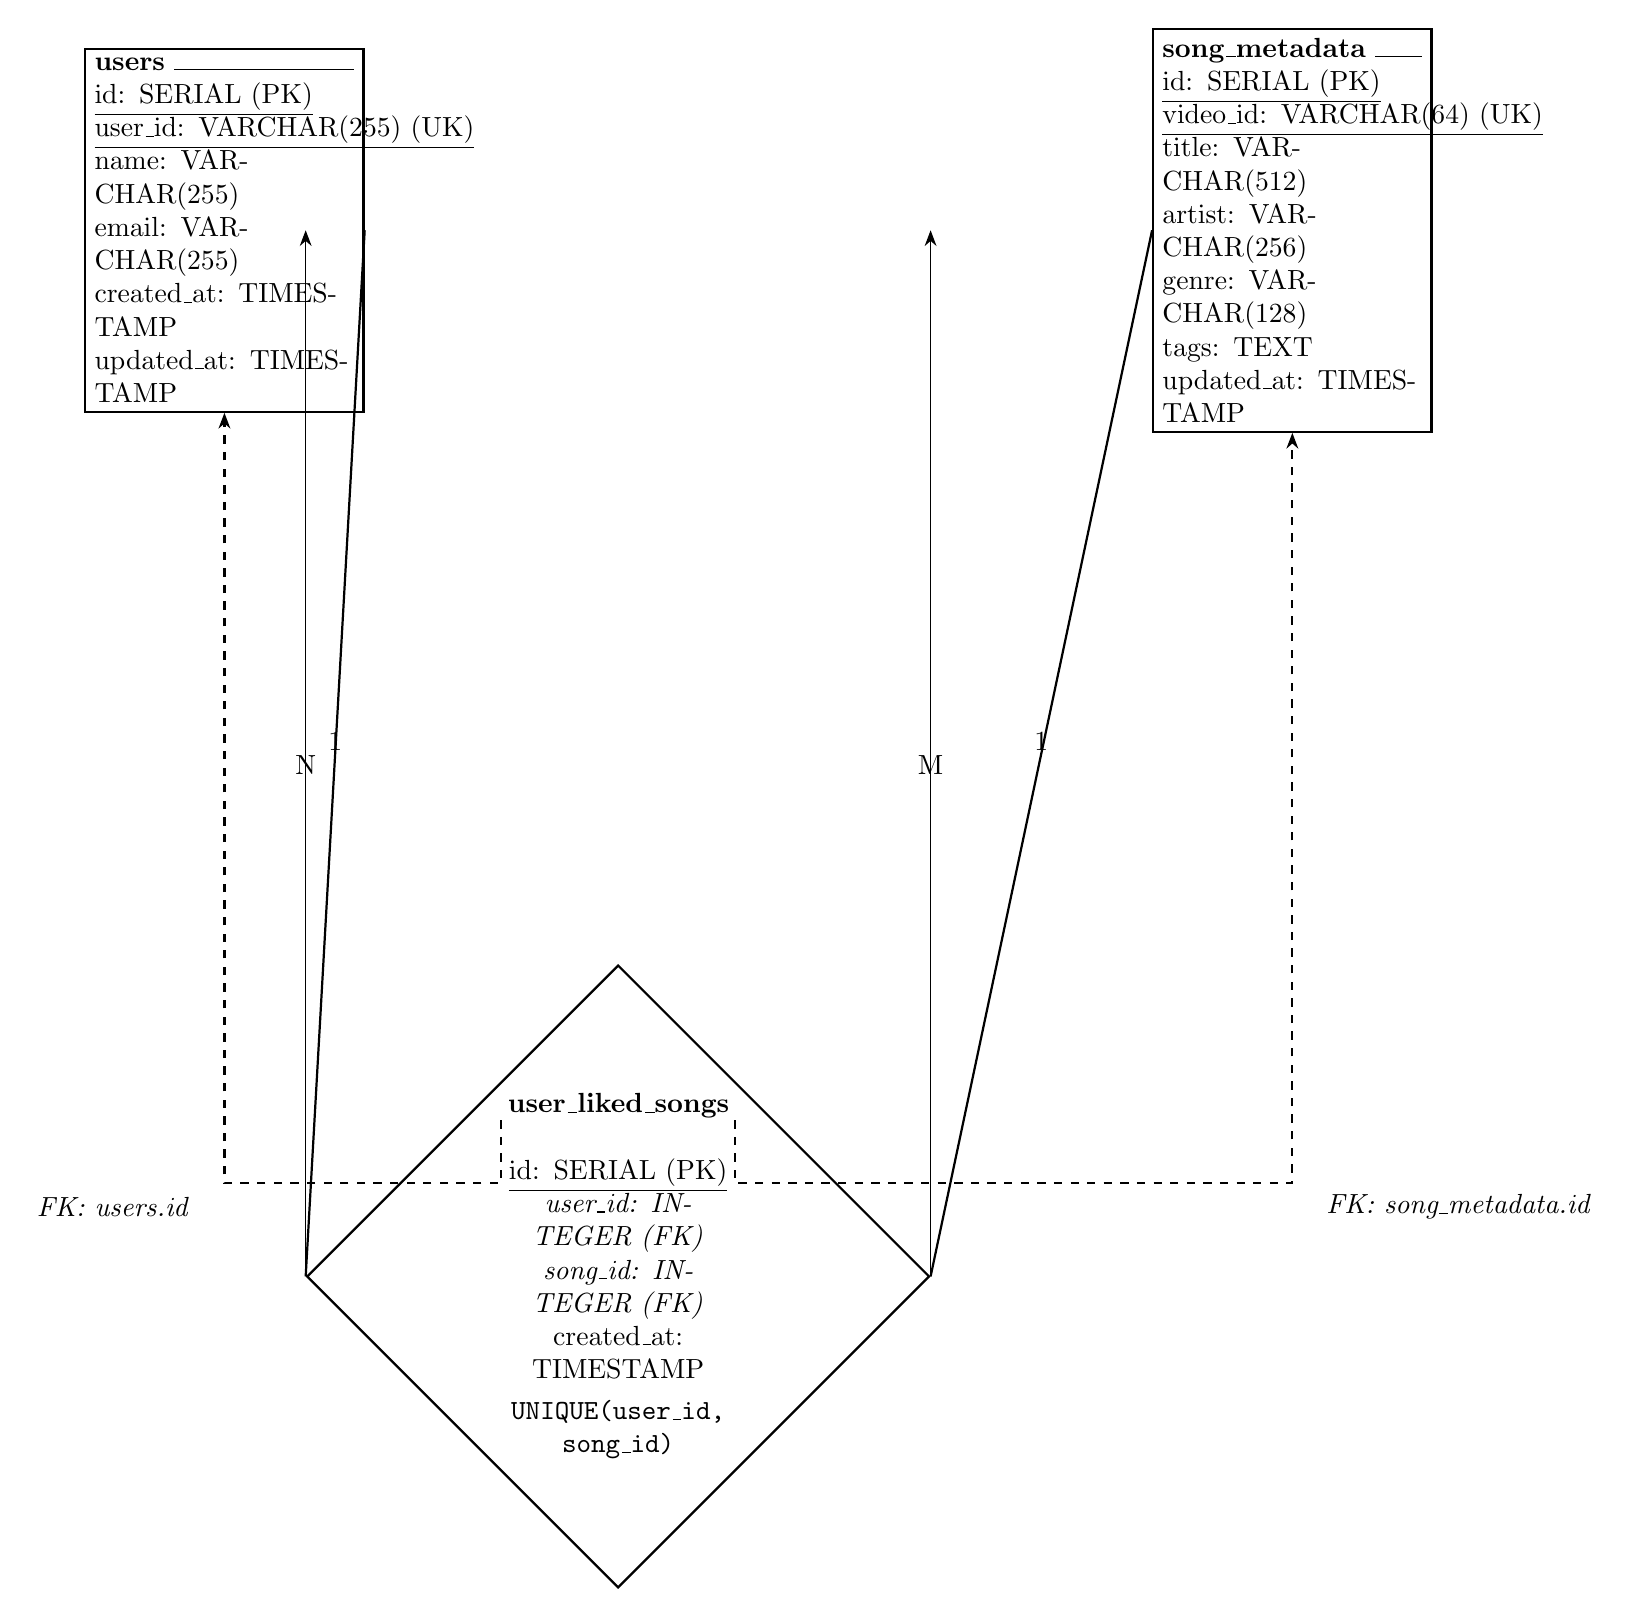
\begin{tikzpicture}[node distance=5cm, auto]
        % Entities
        \node[entity] (user) {
            \textbf{users}
            \hrulefill \\ % Use hrulefill for better line
            \underline{id: SERIAL (PK)} \\
            \underline{user\_id: VARCHAR(255) (UK)} \\
            name: VARCHAR(255) \\
            email: VARCHAR(255) \\
            created\_at: TIMESTAMP \\
            updated\_at: TIMESTAMP
        };
        
        \node[entity] (song) [right=of user, xshift=5cm] {
            \textbf{song\_metadata}
            \hrulefill \\
            \underline{id: SERIAL (PK)} \\
            \underline{video\_id: VARCHAR(64) (UK)} \\
            title: VARCHAR(512) \\
            artist: VARCHAR(256) \\
            genre: VARCHAR(128) \\
            tags: TEXT \\ % Added tags based on migration
            updated\_at: TIMESTAMP
        };
        
        \node[relationship] (likes) [below=of user, yshift=-2cm, xshift=5cm] { % Adjusted position
            \textbf{user\_liked\_songs}
            \hrulefill \\
            \underline{id: SERIAL (PK)} \\
            \textit{user\_id: INTEGER (FK)} \\
            \textit{song\_id: INTEGER (FK)} \\
            created\_at: TIMESTAMP \\
            \vspace{1mm} % Add space before constraint
            \texttt{UNIQUE(user\_id, song\_id)}
        };
        
        % Relationships with Cardinality
        \draw[thick] (user.east) -- node[above=-1mm] {1} (likes.west) node[below=-1mm] {} ; % Adjusted label pos
         \draw[-{Stealth[length=2mm]}] (likes.west) -- node[above=-1mm] {} node[below=-1mm] {N} (user.east -| likes.west) ; % Arrow showing N side

        \draw[thick] (song.west) -- node[above=-1mm] {1} (likes.east) node[below=-1mm] {}; % Adjusted label pos
         \draw[-{Stealth[length=2mm]}] (likes.east) -- node[above=-1mm] {} node[below=-1mm] {M} (song.west -| likes.east) ; % Arrow showing M side

        % Foreign Key Arrows - clearer routing
        \draw[-{Stealth[length=2mm]}, dashed, thick] (likes.north west) ++(0.5,0) -- ++(0,-0.8) -| (user.south) node[midway, left, xshift=-3mm, yshift=-3mm] {\textit{FK: users.id}};
        \draw[-{Stealth[length=2mm]}, dashed, thick] (likes.north east) ++(-0.5,0) -- ++(0,-0.8) -| (song.south) node[midway, right, xshift=3mm, yshift=-3mm] {\textit{FK: song\_metadata.id}};

    \end{tikzpicture}
    \caption{Logical ER Diagram for the TuneTrace schema (Version 2.0). Attributes reflect the state after the \texttt{add\_user\_oauth\_fields.py} migration.}
    \label{fig:er_current}
\end{figure}

\subsection{Physical Model and ORM Mapping}
The logical schema is translated into a physical database schema (SQL table definitions) and mapped to Python classes using the SQLAlchemy ORM. This mapping is defined in \texttt{db.py}, where classes inherit from \texttt{Base = DeclarativeBase()}. SQLAlchemy translates Python object interactions into SQL statements executed against the configured database engine.

\subsubsection{User Model Mapping}
The \texttt{User} class maps to the \texttt{users} table.
\begin{Verbatim}[commandchars=\\\{\}, frame=single]
class User(Base):
    __tablename__ = "users"

    id: Mapped[int] = mapped_column(Integer, primary_key=True, 
                                     autoincrement=True)
    user_id: Mapped[str] = mapped_column(
        String(255), unique=True, index=True,
        comment="User email or unique identifier from OAuth..."
    )
    name: Mapped[Optional[str]] = mapped_column(String(255), nullable=True, ...)
    email: Mapped[Optional[str]] = mapped_column(String(255), nullable=True, 
                                               index=True, ...)
    created_at: Mapped[datetime] = mapped_column(DateTime, 
                                                default=datetime.utcnow)
    updated_at: Mapped[datetime] = mapped_column(DateTime, 
                                                default=datetime.utcnow, 
                                                onupdate=datetime.utcnow)
    # Relationship to UserLikedSong
    likes: Mapped[List["UserLikedSong"]] = relationship(
        "UserLikedSong", back_populates="user", 
        cascade="all, delete-orphan"
    )
    
    def get_liked_song_ids(self) -> Set[int]:
        return \{like.song_id for like in self.likes\}
\end{Verbatim}
Key features:
\begin{itemize}
    \item \texttt{Mapped[...]}: Uses modern SQLAlchemy 2.0 type-annotated mapping.
    \item \texttt{primary\_key=True}, \texttt{autoincrement=True}: Defines the surrogate primary key.
    \item \texttt{unique=True}, \texttt{index=True}: Defines the business key (\texttt{user\_id}) and ensures efficient lookups. An index is also explicitly created for \texttt{email}.
    \item \texttt{relationship(...)}: Defines the one-to-many relationship from \texttt{User} to \texttt{UserLikedSong}. \texttt{back\_populates="user"} links it to the corresponding relationship in \texttt{UserLikedSong}. \texttt{cascade="all, delete-orphan"} ensures that when a \texttt{User} is deleted, all associated \texttt{UserLikedSong} records are also deleted (database-level \texttt{ON DELETE CASCADE} is also defined via ForeignKey for robustness).
    \item \texttt{get\_liked\_song\_ids()}: A helper method leveraging the relationship to retrieve associated song IDs efficiently.
\end{itemize}

\subsubsection{SongMetadata Model Mapping}
The \texttt{SongMetadata} class maps to the \texttt{song\_metadata} table.
\begin{Verbatim}[commandchars=\\\{\}, frame=single]
class SongMetadata(Base):
    __tablename__ = "song_metadata"
    __table_args__ = (UniqueConstraint("video_id", name="uq_video_id"),)

    id: Mapped[int] = mapped_column(Integer, primary_key=True, ...)
    video_id: Mapped[str] = mapped_column(String(64), index=True, ...)
    title: Mapped[str] = mapped_column(String(512))
    artist: Mapped[str] = mapped_column(String(256), ...)
    genre: Mapped[Optional[str]] = mapped_column(String(128), nullable=True, 
                                              index=True)
    tags: Mapped[Optional[str]] = mapped_column(Text, nullable=True, ...)
    updated_at: Mapped[datetime] = mapped_column(DateTime, ..., 
                                                onupdate=datetime.utcnow)
\end{Verbatim}
Key features:
\begin{itemize}
    \item \texttt{\_\_table\_args\_\_}: Defines table-level constraints, here the unique constraint on \texttt{video\_id}.
    \item \texttt{index=True}: Indexes are defined for \texttt{video\_id} (crucial for checking existence) and \texttt{genre} (for fallback queries).
\end{itemize}

\subsubsection{UserLikedSong Model Mapping (Association Table)}
The \texttt{UserLikedSong} class maps to the \texttt{user\_liked\_songs} junction table.
\begin{Verbatim}[commandchars=\\\{\}, frame=single]
class UserLikedSong(Base):
    __tablename__ = "user_liked_songs"
    __table_args__ = (
        UniqueConstraint("user_id", "song_id", name="uq_user_song"),
    )

    id: Mapped[int] = mapped_column(Integer, primary_key=True, ...)
    user_id: Mapped[int] = mapped_column(
        ForeignKey("users.id", ondelete="CASCADE")
    )
    song_id: Mapped[int] = mapped_column(
        ForeignKey("song_metadata.id", ondelete="CASCADE")
    )
    created_at: Mapped[datetime] = mapped_column(DateTime, 
                                                default=datetime.utcnow)
    
    # Relationships back to User and SongMetadata
    user: Mapped["User"] = relationship("User", back_populates="likes")
    song: Mapped["SongMetadata"] = relationship("SongMetadata")
\end{Verbatim}
Key features:
\begin{itemize}
    \item \texttt{ForeignKey(...)}: Defines the foreign key constraints linking to the \texttt{id} columns of the \texttt{users} and \texttt{song\_metadata} tables. The \texttt{ondelete="CASCADE"} directive instructs the database (PostgreSQL) to automatically delete rows in this table if the referenced user or song is deleted, ensuring referential integrity.
    \item \texttt{UniqueConstraint(...)}: Enforces the business rule that a user can like a specific song only once.
    \item \texttt{relationship(...)}: Defines the many-to-one relationships back to the parent tables. \texttt{back\_populates} links the \texttt{user} relationship to the \texttt{likes} relationship in the \texttt{User} class. The \texttt{song} relationship allows easy access to the metadata of the liked song.
\end{itemize}
This ORM mapping provides a Pythonic way to interact with the relational database schema, abstracting away much of the underlying SQL while still allowing for fine-grained control and leveraging database features like constraints and cascades.

% --- V. DATA MANAGEMENT ---
\section{Data Management and Operations}
The management of data within TuneTrace, including creation, retrieval, and updates, is primarily handled by the \texttt{MusicRepository} class. This class acts as an abstraction layer over the SQLAlchemy session, encapsulating data access logic. The underlying PostgreSQL database guarantees data integrity and consistency through ACID properties, managed via SQLAlchemy's transaction handling.

\subsection{Transaction Management and ACID Properties}
SQLAlchemy's \texttt{Session} object manages database transactions, ensuring that operations adhere to the ACID principles (Atomicity, Consistency, Isolation, Durability), which are fundamental properties guaranteed by transactional databases like PostgreSQL \cite{3}.
\begin{itemize}
    \item \textbf{Atomicity:} Ensures that all operations within a single transaction are treated as a single, indivisible unit. In TuneTrace, when processing a \texttt{POST /suggestions} request, the operations of potentially creating a user, potentially creating song metadata entries, and creating multiple \texttt{UserLikedSong} entries are typically performed within one transaction block. The final call to \texttt{db.commit()} within \texttt{MusicRepository.persist\_user\_likes} attempts to make all these changes permanent. If any operation within this scope fails (e.g., due to a unique constraint violation on \texttt{user\_liked\_songs} or a database connection error), the session automatically rolls back *all* changes made since the last commit, ensuring the database state remains unchanged, as if the transaction never occurred.
    \item \textbf{Consistency:} Guarantees that a transaction brings the database from one valid state to another, preserving data integrity rules defined by constraints. The schema constraints defined in the ORM models and enforced by PostgreSQL (Primary Keys, Foreign Keys with \texttt{ON DELETE CASCADE}, Unique Constraints like \texttt{uq\_user\_song}) ensure this. For example, the system prevents the creation of a "like" referencing a non-existent user or song (FK constraint) and prevents duplicate "likes" (Unique constraint).
    \item \textbf{Isolation:} Ensures that concurrent transactions do not interfere with each other, making them appear as if they execute sequentially. PostgreSQL's default transaction isolation level is \texttt{READ COMMITTED}, which SQLAlchemy sessions typically inherit. This level guarantees that a transaction will only see data that has been committed before it began and will not see uncommitted changes ("dirty reads") from other concurrent transactions. While sufficient for many applications, higher levels like \texttt{REPEATABLE READ} or \texttt{SERIALIZABLE} could be configured if stricter isolation is needed, though potentially at the cost of reduced concurrency. The \texttt{get\_or\_create\_user} method includes basic handling for a potential race condition where two requests might try to create the same user simultaneously.
    \item \textbf{Durability:} Ensures that once a transaction has been successfully committed (\texttt{db.commit()} returns without error), its changes are permanent and will survive subsequent system failures (e.g., crashes, power outages). PostgreSQL achieves this through mechanisms like Write-Ahead Logging (WAL), where changes are first written to a persistent log before being applied to the data files \cite{5}.
\end{itemize}
The \texttt{get\_session} dependency in \texttt{main.py} manages the lifecycle of the session for each request, ensuring \texttt{db.close()} is called, which typically handles rollback on error or releasing the connection back to the pool after a successful commit.

\subsection{Write Operation Implementation (\texttt{POST /suggestions})}
The primary write operation occurs when a user submits a list of liked songs via the \texttt{POST /suggestions} endpoint. The process involves several steps orchestrated between the endpoint handler, the \texttt{SuggestionService}, and the \texttt{MusicRepository}:

1.  \textbf{User Identification/Creation:} The \texttt{MusicRepository.get\_or\_create\_user} method is called with the \texttt{user\_id} (OAuth email) from the request.
    \begin{Verbatim}[commandchars=\\\{\}, frame=single]
# From main.py: MusicRepository class
def get_or_create_user(self, user_id: str) -> User:
    # Attempt to find existing user, eager load likes
    user = self.db.query(User).options(
        joinedload(User.likes) 
    ).filter_by(user_id=user_id).one_or_none()
    
    if not user:
        user = User(user_id=user_id) # Create new User object
        self.db.add(user) # Add to session
        try:
            self.db.flush() # Send INSERT to DB, get generated ID
        except Exception: # Handle potential race condition
            self.db.rollback() # Rollback the failed insert attempt
            # Re-fetch the user presumably created by another request
            user = self.db.query(User).options(
                joinedload(User.likes)
            ).filter_by(user_id=user_id).one()
    return user
    \end{Verbatim}
    This method performs an "upsert" (update or insert) logic. It first queries for the user. If not found, it creates a new \texttt{User} instance, adds it to the session, and calls \texttt{db.flush()}. Flushing sends pending SQL (the \texttt{INSERT}) to the database and retrieves the generated primary key (\texttt{user.id}) without ending the transaction. The \texttt{try...except} block handles potential race conditions if two requests try creating the same user concurrently. \texttt{joinedload(User.likes)} is used to efficiently pre-load the user's existing likes in the same query, avoiding potential N+1 query problems later.

2.  \textbf{Song Resolution and Persistence:} For each song name in the request's \texttt{songs} list, the \texttt{SuggestionService.\_search\_youtube\_for\_song(song\_name)} method is called. This method (using \texttt{@lru\_cache}) queries the YouTube API to get the \texttt{video\_id}, title, and artist.
    Once the \texttt{video\_id} is obtained, the repository's \texttt{get\_song\_metadata\_by\_video\_id(video\_id)} method checks if the song already exists in the database.
    If the song is not found, \texttt{MusicRepository.create\_song\_metadata(video\_data)} is called:
    \begin{Verbatim}[commandchars=\\\{\}, frame=single]
# From main.py: MusicRepository class
def create_song_metadata(self, video_data: dict) -> SongMetadata:
    song = SongMetadata(
        video_id=video_data["video_id"],
        title=video_data["title"],
        artist=video_data["artist"],
        # Genre/Tags might be added here if available
    )
    self.db.add(song) # Add to session
    self.db.flush() # Send INSERT, get generated ID
    return song
    \end{Verbatim}
    This creates a new \texttt{SongMetadata} record. Again, \texttt{db.flush()} retrieves the new \texttt{song\_meta.id}. A set of unique internal song IDs (\texttt{song\_metadata\_ids\_to\_like}) corresponding to the user's input is collected.

3.  \textbf{Persisting Likes:} Finally, \texttt{MusicRepository.persist\_user\_likes} is called with the retrieved \texttt{User} object and the set of song IDs.
    \begin{Verbatim}[commandchars=\\\{\}, frame=single]
# From main.py: MusicRepository class
def persist_user_likes(self, 
                       user: User, 
                       song_metadata_ids: Set[int]):
    # Get IDs already liked by the user (loaded via joinedload)
    existing_liked_ids = \{like.song_id for like in user.likes\}
    # Determine which new IDs need to be added
    ids_to_add = song_metadata_ids - existing_liked_ids
    
    if ids_to_add:
        # Create UserLikedSong objects for new likes
        new_likes = [
            UserLikedSong(user_id=user.id, song_id=song_id) 
            for song_id in ids_to_add
        ]
        self.db.add_all(new_likes) # Add multiple objects efficiently
    
    self.db.commit() # Commit the entire transaction
    \end{Verbatim}
    This method efficiently determines which of the submitted likes are new by comparing against the pre-loaded \texttt{existing\_liked\_ids}. It creates \texttt{UserLikedSong} objects only for the new likes and uses \texttt{db.add\_all} for potentially bulk insertion. The crucial \texttt{db.commit()} call finalizes the transaction, making all changes (user creation, song creation, like creation) durable.

4.  \textbf{Background Cache Update:} After successfully committing to the database, the endpoint schedules a background task (\texttt{background\_tasks.add\_task(update\_redis\_user\_likes, ...)}) to update the Redis cache asynchronously. This ensures the user's API response is not delayed by the cache write operation.

\subsection{Read Operation Implementation}
The primary read operations involve fetching a user's liked songs (\texttt{GET /liked-songs}) and generating recommendations (\texttt{POST /suggestions}).

1.  \textbf{Fetching Liked Songs (\texttt{GET /liked-songs}):} This is handled by \texttt{MusicRepository.get\_user\_liked\_songs}.
    \begin{Verbatim}[commandchars=\\\{\}, frame=single]
# From main.py: MusicRepository class
def get_user_liked_songs(self, user_id: str) -> List[tuple]:
    user = self.db.query(User).filter_by(user_id=user_id).one_or_none()
    if not user: return []
    
    results = (
        self.db.query(
            SongMetadata.video_id,
            SongMetadata.title,
            SongMetadata.artist,
            UserLikedSong.created_at
        )
        .join(UserLikedSong, UserLikedSong.song_id == SongMetadata.id)
        .filter(UserLikedSong.user_id == user.id)
        .order_by(UserLikedSong.created_at.desc())
        .all()
    )
    return results
    \end{Verbatim}
    This method first finds the user by their external \texttt{user\_id}. If found, it executes a query that joins \texttt{SongMetadata} with \texttt{UserLikedSong} based on the user's internal \texttt{id}, filters for that user, selects the required metadata fields, orders the results by the like timestamp, and returns them.

2.  \textbf{Generating Collaborative Suggestions:} This is the most complex query, executed within \texttt{MusicRepository.get\_collaborative\_suggestions} after the write operations in \texttt{POST /suggestions}.
    \begin{Verbatim}[commandchars=\\\{\}, frame=single]
# From main.py: MusicRepository class
def get_collaborative_suggestions(self, 
                                user: User, 
                                limit: int = 10) -> List[SongMetadata]:
    if not user.likes: return [] # Check if user has likes
    
    user_liked_song_ids = user.get_liked_song_ids() # Set of IDs
    
    # Step 1: Find IDs of similar users
    similar_users_query = (
        self.db.query(User.id) # Select only the user ID
        .join(UserLikedSong) # Join users with their likes
        # Filter likes to those matching the current user's likes
        .filter(UserLikedSong.song_id.in_(user_liked_song_ids)) 
        .filter(User.id != user.id) # Exclude the current user
        .group_by(User.id) # Group by user to count common songs
        # Having clause: require at least 2 common songs
        .having(func.count(UserLikedSong.song_id) >= 2) 
    )
    similar_users = similar_users_query.all() # Execute query
    
    if not similar_users: return [] # No similar users found
    
    similar_user_ids = [u[0] for u in similar_users] # Extract IDs
    
    # Step 2: Get recommendations based on similar users' likes
    recommendations_query = (
        self.db.query(SongMetadata) # Select full SongMetadata objects
        .join(UserLikedSong) # Join songs with likes
        # Filter likes to only those by similar users
        .filter(UserLikedSong.user_id.in_(similar_user_ids)) 
        # Filter out songs the current user already likes
        .filter(~SongMetadata.id.in_(user_liked_song_ids)) 
        .group_by(SongMetadata.id) # Group by song
        # Order by the count of similar users who liked this song
        .order_by(func.count(UserLikedSong.user_id).desc()) 
        .limit(limit) # Limit the number of results
    )
    recommendations = recommendations_query.all() # Execute query
    
    return recommendations
    \end{Verbatim}
    This method breaks down the collaborative filtering logic into two main database queries executed via the ORM:
    \begin{itemize}
        \item \textbf{Find Similar Users:} It joins \texttt{users} and \texttt{user\_liked\_songs}, filters for songs also liked by the current user (\texttt{UserLikedSong.song\_id.in\_(...)}) while excluding the current user themselves. It then groups by \texttt{User.id} and uses a \texttt{HAVING} clause with \texttt{func.count()} to find only those users who share at least two songs in common. This query efficiently identifies the "neighbors".
        \item \textbf{Generate Recommendations:} It joins \texttt{song\_metadata} and \texttt{user\_liked\_songs}, filtering for likes made only by the identified \texttt{similar\_user\_ids}. Crucially, it filters out songs the current user has already liked (\texttt{\~SongMetadata.id.in\_(...)}). It groups by song and orders the results by the count of distinct similar users who liked each song (\texttt{func.count(UserLikedSong.user\_id).desc()}), effectively ranking suggestions by popularity within the similar user group. Finally, it limits the results.
    \end{itemize}
    SQLAlchemy translates these expressive ORM queries into optimized SQL, leveraging joins, filtering, aggregation (\texttt{GROUP BY}, \texttt{COUNT}), and ordering to perform the core recommendation logic directly within the database engine.

% --- VI. PERFORMANCE OPTIMIZATION ---
\section{Performance Optimization}
Delivering timely recommendations requires optimizing database queries and minimizing latency, especially for the potentially complex collaborative filtering operation and external API calls. TuneTrace employs several standard optimization techniques.

\subsection{Indexing Strategy}
Database indexes are crucial data structures that allow the DBMS (PostgreSQL) to locate rows matching query conditions much faster than scanning entire tables. The TuneTrace schema and SQLAlchemy models define several indexes, primarily B-Trees, which are effective for equality and range queries \cite{3, 5}.
\begin{itemize}
    \item \textbf{Primary Key Indexes:} PostgreSQL automatically creates unique B-Tree indexes on the primary key columns: \texttt{users(id)}, \texttt{song\_metadata(id)}, and \texttt{user\_liked\_songs(id)}. These guarantee uniqueness and provide the fastest way to access a specific row by its internal ID.
    \item \textbf{Unique Key Indexes:} Unique constraints also typically create underlying unique indexes. In TuneTrace, these are:
        \begin{itemize}
            \item \texttt{users(user\_id)}: Essential for quickly finding a user based on their external identifier (OAuth email) in \texttt{get\_or\_create\_user}.
            \item \texttt{song\_metadata(video\_id)}: Crucial for efficiently checking if a song fetched from YouTube already exists in the database (\texttt{get\_song\_metadata\_by\_video\_id}).
            \item \texttt{user\_liked\_songs(user\_id, song\_id)}: This composite unique index enforces the "like once" rule and significantly speeds up checks in \texttt{persist\_user\_likes} to avoid inserting duplicates. Importantly, this multi-column index can also efficiently serve queries filtering only on \texttt{user\_id} (its leading column).
        \end{itemize}
    \item \textbf{Foreign Key Indexing:} While not strictly required by SQL standards, it's a best practice to index foreign key columns, and SQLAlchemy typically encourages this. PostgreSQL often benefits greatly from indexes on FK columns involved in joins. The composite index on \texttt{user\_liked\_songs(user\_id, song\_id)} implicitly helps queries joining on \texttt{user\_id}. An explicit index on \texttt{user\_liked\_songs(song\_id)} would further optimize joins from \texttt{song\_metadata} or queries filtering primarily by song. The collaborative filtering query heavily relies on joins involving \texttt{user\_liked\_songs.user\_id} and \texttt{user\_liked\_songs.song\_id}, making indexing here critical for performance. The initial migration explicitly creates indexes: \texttt{ix\_users\_user\_id} and \texttt{ix\_song\_metadata\_video\_id}. The unique constraint on \texttt{user\_liked\_songs} provides indexing benefits.
    \item \textbf{Attribute Indexes:} Indexes can also be created on non-key attributes frequently used in \texttt{WHERE} clauses or \texttt{ORDER BY} clauses.
        \begin{itemize}
            \item \texttt{users(email)}: An index is explicitly created on the \texttt{email} field in the \texttt{add\_user\_oauth\_fields.py} migration, anticipating potential lookups by email address.
            \item \texttt{song\_metadata(genre)}: An index is created on the \texttt{genre} field, as specified in the initial migration (\texttt{ix\_song\_metadata\_genre}). While not used by the primary collaborative filtering algorithm, this index is vital for the performance of the content-based fallback mechanism (\texttt{\_get\_fallback\_suggestions}), which might filter or search based on genre.
        \end{itemize}
\end{itemize}
These indexes allow the PostgreSQL query planner to choose more efficient execution plans (e.g., index scans, index-only scans, faster join methods like hash joins or merge joins) instead of resorting to slow sequential scans of large tables, especially as the number of users, songs, and likes grows.

\subsection{Caching Subsystem}
Caching is employed to store frequently accessed or computationally expensive data in faster storage tiers (memory) to reduce response times and lessen the load on slower tiers (database, external APIs). TuneTrace uses a multi-layer caching approach \cite{6}.

\begin{enumerate}
    \item \textbf{Redis Cache (Distributed L2 Cache):} Configured via the \texttt{REDIS\_URL} environment variable. Redis is an in-memory key-value store known for its speed \cite{6}.
        \begin{itemize}
            \item \textbf{Usage:} Primarily intended to cache user preference data (specifically, the set of liked song IDs). The function \texttt{update\_redis\_user\_likes} is responsible for this.
            \item \textbf{Strategy (Write-Aside/Background Update):} When likes are persisted to PostgreSQL (\texttt{persist\_user\_likes}), a FastAPI \texttt{BackgroundTasks} instance is used to schedule \texttt{update\_redis\_user\_likes}. This function runs *after* the HTTP response has been sent to the client. It takes the user's ID and the set of their liked song IDs, serializes the set into a JSON string (\texttt{json.dumps(list(song\_ids))}), and stores it in Redis under a key like \texttt{user\_likes:\{user\_id\}}. This makes the primary database write synchronous (ensuring durability) but the cache update asynchronous (improving API response time).
            \item \textbf{TTL (Time-To-Live):} A TTL is set on the cached data using the \texttt{REDIS\_TTL\_SECONDS} environment variable (defaulting to 3600 seconds / 1 hour). This ensures cached data eventually expires, forcing a refresh from the primary database and preventing stale data from persisting indefinitely.
            \item \textbf{Graceful Degradation:} The code checks if \texttt{redis\_client} is available before attempting operations. If Redis is unavailable (e.g., connection error, not configured), it logs a warning but allows the application to continue functioning, likely relying on the database or other cache layers, thus providing resilience.
        \end{itemize}
    \item \textbf{In-Memory LRU Cache (Application L1 Cache):} Implemented using Python's built-in \texttt{functools.lru\_cache} decorator.
        \begin{itemize}
            \item \textbf{Usage:} Applied directly to the \texttt{SuggestionService.\_search\_youtube\_for\_song} method: \texttt{@lru\_cache(maxsize=512)}.
            \item \textbf{Functionality:} This caches the return values of the \texttt{\_search\_youtube\_for\_song} function based on its input arguments (the \texttt{song\_name} string). When the same song name is searched again within the same application process, the cached result (the dictionary containing \texttt{video\_id}, \texttt{title}, \texttt{artist}) is returned instantly without calling the YouTube API.
            \item \textbf{Strategy (Least Recently Used):} The \texttt{maxsize=512} parameter limits the cache to storing the results of the 512 most recent unique song searches. When the cache is full and a new song is searched, the least recently used entry is evicted.
            \item \textbf{Benefits:} Significantly reduces the number of calls to the external YouTube Data API, which saves costs (API quotas), reduces latency associated with network requests, and makes the application less dependent on the external service's availability.
        \end{itemize}
\end{enumerate}
This combination of a distributed cache for user data and a local in-memory cache for external API results provides substantial performance benefits and improves the application's resilience.

% --- VII. DATABASE EVOLUTION ---
\section{Database Evolution (Schema Migrations)}
As applications evolve, their database schemas often need to change to accommodate new features, fix design flaws, or improve performance. Managing these changes in a controlled, versioned, and reversible manner is crucial, especially in production environments. TuneTrace utilizes \textbf{Alembic}, a popular database migration tool for SQLAlchemy, to handle schema evolution \cite{4}.

\subsection{Alembic Configuration}
Alembic's behavior is configured through the \texttt{alembic.ini} file and the \texttt{alembic/env.py} script.
\begin{itemize}
    \item \textbf{\texttt{alembic.ini}:}
        \begin{itemize}
            \item \texttt{script\_location = alembic}: Specifies the directory containing migration scripts.
            \item \texttt{sqlalchemy.url = \%(POSTGRES\_DATABASE\_URL)s}: This key line configures the target database connection. It uses Python's string interpolation syntax (\texttt{\%...\%}s) to instruct Alembic to read the actual database URL from the \texttt{POSTGRES\_DATABASE\_URL} environment variable at runtime. This avoids hardcoding credentials and allows the same configuration to work across different environments (development, staging, production) by simply setting the appropriate environment variable.
            \item Logging sections ([\texttt{loggers}], [\texttt{handlers}], etc.): Configure how Alembic logs its operations.
        \end{itemize}
    \item \textbf{\texttt{alembic/env.py}:} This script is executed whenever an Alembic command is run. It bridges the gap between Alembic and the application's SQLAlchemy models.
        \begin{itemize}
            \item **Python Path Setup:** It modifies \texttt{sys.path} to ensure Alembic can import the application's models (\texttt{from db import Base}).
            \item **Environment Loading:** It uses \texttt{load\_dotenv()} to load environment variables from a \texttt{.env} file, which is particularly useful for local development when running Alembic commands from the terminal.
            \item **Database URL Handling:** It reads the \texttt{POSTGRES\_DATABASE\_URL} environment variable. If it's not set (typical in local development without a dedicated Postgres instance), it defaults to the SQLite URL (\texttt{sqlite:///./app.db}) and sets this URL back into Alembic's configuration using \texttt{config.set\_main\_option("sqlalchemy.url", DATABASE\_URL)}. This ensures Alembic commands can run locally even without a production database environment.
            \item **Metadata Binding:** It sets \texttt{target\_metadata = Base.metadata}. This crucial step tells Alembic which SQLAlchemy models define the target state of the database schema. Alembic uses this metadata to compare against the current database state and to auto-generate migration scripts.
            \item **Migration Execution Logic:** It defines \texttt{run\_migrations\_offline()} (generates SQL scripts) and \texttt{run\_migrations\_online()} (connects to the database and applies changes). The online mode uses \texttt{engine\_from\_config} which reads the \texttt{sqlalchemy.url} set earlier.
        \end{itemize}
\end{itemize}
This setup provides a flexible and environment-aware configuration for managing database migrations.

\subsection{Migration Implementation Examples}
The \texttt{alembic/versions} directory contains the individual migration scripts, each representing a step in the schema's evolution. Two examples are provided:

\begin{enumerate}
    \item \textbf{Initial Schema Creation (\texttt{999777df0f65\_create\_initial\_tables.py}):}
        \begin{itemize}
            \item \textbf{Purpose:} Defines the initial database schema (Version 1.0).
            \item \textbf{\texttt{upgrade()} Function:} Uses Alembic's operation directives (\texttt{op}) to create the necessary tables:
                \begin{itemize}
                    \item \texttt{op.create\_table('users', ...)}: Defines columns (\texttt{id}, \texttt{user\_id}, \texttt{created\_at}) with types, constraints (PK), and comments.
                    \item \texttt{op.create\_table('song\_metadata', ...)}: Defines columns (\texttt{id}, \texttt{video\_id}, \texttt{title}, \texttt{artist}, \texttt{genre}, \texttt{tags}, \texttt{updated\_at}) with constraints (PK, UK) and comments.
                    \item \texttt{op.create\_table('user\_liked\_songs', ...)}: Defines columns (\texttt{id}, \texttt{user\_id}, \texttt{song\_id}, \texttt{created\_at}) with constraints (PK, UK on user/song pair) and foreign key references (\texttt{sa.ForeignKeyConstraint}) including the \texttt{ondelete='CASCADE'} rule.
                    \item \texttt{op.create\_index(...)}: Explicitly creates indexes on \texttt{users.user\_id}, \texttt{song\_metadata.video\_id}, and \texttt{song\_metadata.genre}. Note that indexes for PKs and UKs are often created automatically by the DB.
                \end{itemize}
            \item \textbf{\texttt{downgrade()} Function:} Contains the inverse operations (\texttt{op.drop\_table}, \texttt{op.drop\_index}) to revert the schema back to its state before this migration was applied. This allows for controlled rollbacks.
        \end{itemize}
    \item \textbf{Adding OAuth Fields (\texttt{add\_user\_oauth\_fields.py}):}
        \begin{itemize}
            \item \textbf{Purpose:} Modifies the schema to support OAuth integration and store more user information (Version 2.0). Revision ID \texttt{a1b2c3d4e5f6} revises the initial migration (\texttt{down\_revision = '999777df0f65'}).
            \item \textbf{\texttt{upgrade()} Function:} Uses \texttt{op} directives to modify the existing schema:
                \begin{itemize}
                    \item \texttt{op.add\_column('users', sa.Column('name', ...))}: Adds the optional \texttt{name} column.
                    \item \texttt{op.add\_column('users', sa.Column('email', ...))}: Adds the optional \texttt{email} column.
                    \item \texttt{op.add\_column('users', sa.Column('updated\_at', ...))}: Adds the \texttt{updated\_at} timestamp column, using \texttt{server\_default=sa.func.now()} for database-generated defaults.
                    \item \texttt{op.alter\_column('users', 'user\_id', type\_=sa.String(255), ...)}: Modifies the \texttt{user\_id} column, increasing its length from 128 to 255 characters to reliably store email addresses.
                    \item \texttt{op.create\_index(op.f('ix\_users\_email'), 'users', ['email'], ...)}: Creates a non-unique index on the new \texttt{email} column to speed up potential lookups. The \texttt{op.f()} function provides a consistent naming convention for constraints and indexes.
                \end{itemize}
            \item \textbf{\texttt{downgrade()} Function:} Contains the corresponding \texttt{op.drop\_index}, \texttt{op.alter\_column} (changing type back), and \texttt{op.drop\_column} operations to reverse these changes.
        \end{itemize}
\end{enumerate}
Using Alembic allows developers to manage schema changes alongside code changes in version control (Git), apply migrations consistently across different environments, and safely upgrade or downgrade the database structure as the application evolves. Commands like \texttt{alembic upgrade head} apply all pending migrations, while \texttt{alembic downgrade -1} reverts the last applied migration.

% --- VIII. FUTURE WORK ---
\section{Future Work and Schema Extensions}
While the current TuneTrace schema (Version 2.0) effectively supports the core functionality of user-based collaborative filtering and basic metadata storage, future development to enhance features or improve data quality would necessitate schema extensions. Extended Entity-Relationship (EER) modeling concepts, such as enhanced specialization/generalization and relationship types, can guide these extensions \cite{3}.

\subsection{Artist and Genre Normalization}
A significant limitation of the current schema is the denormalization of artist and genre information. The \texttt{artist} (channel name) and \texttt{genre} are stored as simple string fields directly within the \texttt{song\_metadata} table. This approach suffers from several drawbacks:
\begin{itemize}
    \item \textbf{Data Redundancy:} The same artist name or genre string is repeated for every song associated with it.
    \item \textbf{Inconsistency Issues:} Typos or variations in naming (e.g., "The Beatles" vs. "Beatles") can lead to fragmented data, making it difficult to query accurately (e.g., "find all songs by The Beatles").
    \item \textbf{Limited Querying Power:} It's difficult to perform queries focused on artists or genres themselves (e.g., "find artists similar to X," "list all genres available," "find users who like genre Y").
    \item \textbf{Many-to-Many Artist Relationship:} A song can potentially have multiple artists (collaborations). Storing this as a single string is inadequate.
\end{itemize}

A more robust design involves normalizing this information by creating separate entities for \texttt{Artists} and \texttt{Genres}, as depicted in the proposed ER diagram (Figure \ref{fig:er_normalized}).

\begin{figure}[ht]
    \centering % Center the figure environment content
    \begin{tikzpicture}[node distance=4cm, auto]
        % Entities
        \node[entity] (artist) {
            \textbf{artists}
            \hrulefill \\
            \underline{id: SERIAL (PK)} \\
            name: VARCHAR(256) (UK) \\
            (other artist attributes...)
        };
        
        \node[entity] (song) [right=of artist, xshift=5cm] { % Increased shift
            \textbf{song\_metadata}
            \hrulefill \\
            \underline{id: SERIAL (PK)} \\
            \underline{video\_id: VARCHAR(64) (UK)} \\
            title: VARCHAR(512) \\
            \textit{genre\_id: INTEGER (FK)} \\ % FK to genres
            (other song attributes...)
        };
        
        \node[entity] (genre) [right=of song, xshift=5cm] { % Increased shift
            \textbf{genres}
            \hrulefill \\
            \underline{id: SERIAL (PK)} \\
            name: VARCHAR(128) (UK)
        };
        
        % Junction table for M:N song <-> artist
        \node[relationship] (performs) [below=of song, yshift=-1.5cm] { 
            \textbf{song\_artists}
            \hrulefill \\
            \underline{\textit{song\_id: INTEGER (PK, FK)}} \\
            \underline{\textit{artist\_id: INTEGER (PK, FK)}} \\
            role: VARCHAR(50) % e.g., 'main', 'featured'
        };
        
        % Relationships
        % M:N between Song and Artist via song_artists
        \draw[thick] (artist.south) -- node[midway, left] {1} (performs.west) node[midway, right] {N};
        \draw[thick] (song.south) -- node[midway, right] {1} (performs.east) node[midway, left] {M};
        
        % 1:N between Genre and Song
        \draw[thick] (genre.west) -- node[midway, above] {1} (song.east) node[midway, below] {N};
        
        % Foreign Key Arrows - clearer routing
        \draw[-{Stealth[length=2mm]}, dashed, thick] (performs.north -| artist.south) ++(-0.8,0) -- (artist.south) node[midway, left, xshift=-3mm] {\textit{FK: artists.id}};
        \draw[-{Stealth[length=2mm]}, dashed, thick] (performs.north) -- (song.south) node[midway, right, xshift=3mm] {\textit{FK: song\_metadata.id}};
        \draw[-{Stealth[length=2mm]}, dashed, thick] (song.east) -- (genre.west) node[midway, above, yshift=2mm] {\textit{FK: genres.id}};

    \end{tikzpicture}
    \caption{Proposed normalized schema for Artists and Genres. Introduces \texttt{artists} and \texttt{genres} tables, resolves the M:N song-artist relationship via \texttt{song\_artists}, and links songs to genres via a foreign key.}
    \label{fig:er_normalized}
\end{figure}

In this revised schema:
\begin{itemize}
    \item The \texttt{artists} table stores canonical artist information (unique ID, name).
    \item The \texttt{genres} table stores canonical genre information (unique ID, name).
    \item The \texttt{song\_metadata} table replaces the \texttt{artist} string with potentially multiple links via the \texttt{song\_artists} junction table and replaces the \texttt{genre} string with a foreign key \texttt{genre\_id} referencing the \texttt{genres} table (assuming a song primarily belongs to one genre, or potentially another M:N relationship if multiple genres per song are needed).
    \item The \texttt{song\_artists} table resolves the M:N relationship between songs and artists, allowing a song to be linked to multiple artists and vice-versa. It uses a composite primary key (\texttt{song\_id}, \texttt{artist\_id}) and could include additional attributes describing the relationship (e.g., role like 'main artist', 'featured artist').
\end{itemize}
This normalized structure eliminates redundancy, improves data consistency, and enables more sophisticated querying and analysis based on artists and genres, significantly enhancing the potential for content-based or hybrid recommendation features. Implementing this would require new Alembic migrations to create the tables and potentially migrate existing denormalized data.

\subsection{Extended ER Model: User Specialization for Freemium Model}
To introduce different tiers of service (e.g., free vs. premium users), EER concepts like specialization and generalization can be applied. The current \texttt{users} table can be treated as a **superclass**, containing attributes common to all users. Specific attributes related to different user types can be stored in **subclass** entities.

Figure \ref{fig:er_eer} illustrates a possible specialization hierarchy for a freemium model.

\begin{figure}[H] % Use [H] from float package for 'here' placement
    \centering % Center the figure environment content
    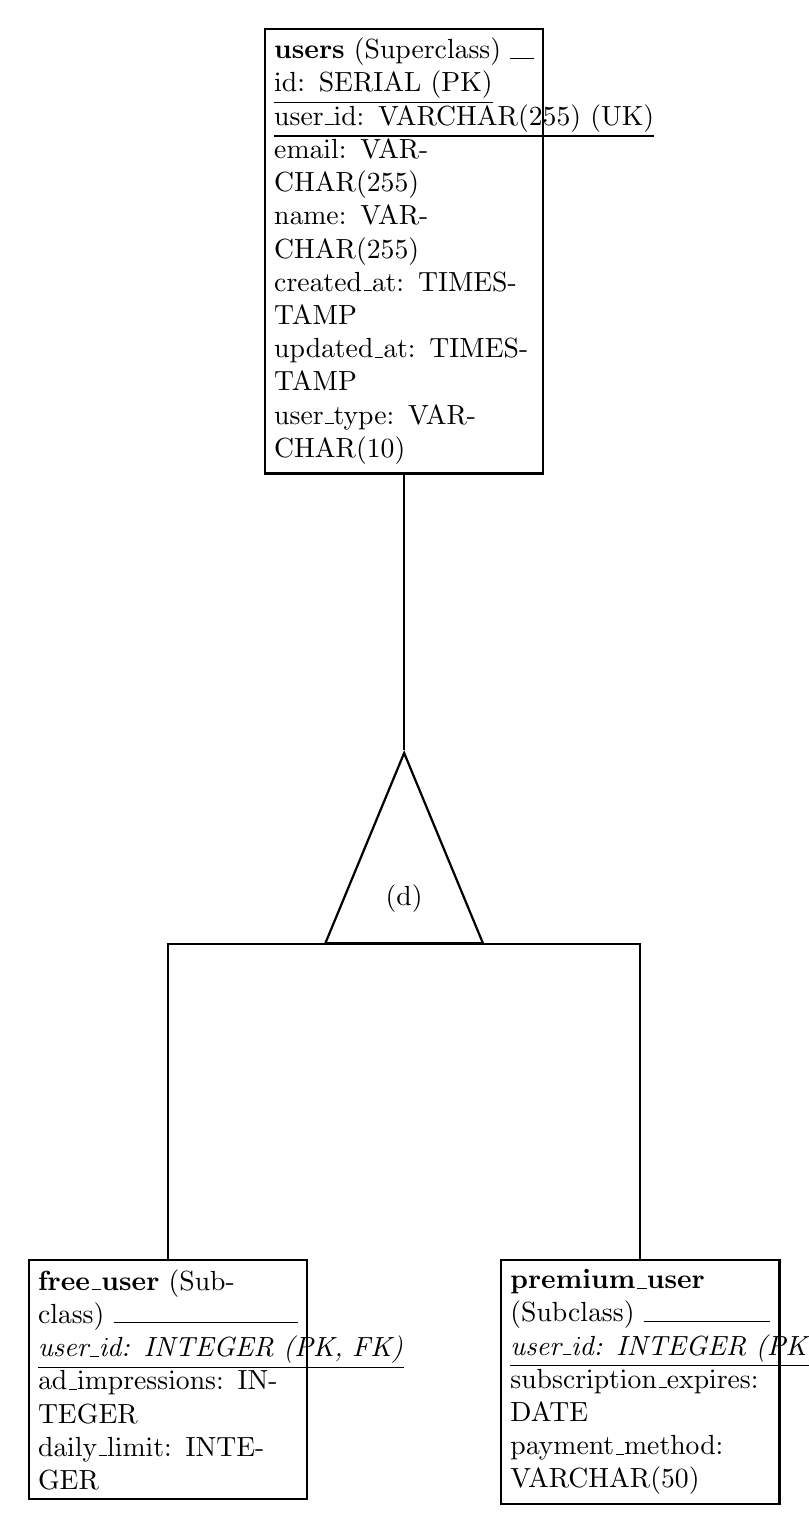
\begin{tikzpicture}[node distance=3cm, auto]
        % Superclass Entity
        \node[entity] (user) {
            \textbf{users} (Superclass)
            \hrulefill \\
            \underline{id: SERIAL (PK)} \\
            \underline{user\_id: VARCHAR(255) (UK)} \\
            email: VARCHAR(255) \\
            name: VARCHAR(255) \\
            created\_at: TIMESTAMP \\
            updated\_at: TIMESTAMP \\
            user\_type: VARCHAR(10) % Discriminator
        };
        
        % ISA Relationship symbol with constraint
        \node[isa] (isa) [below=of user, yshift=-0.5cm] {(d)}; % (d) for disjoint

        % Subclass Entities
        \node[entity] (free) [below=of isa, xshift=-3cm, yshift=-1cm] { % Increased shift
            \textbf{free\_user} (Subclass)
            \hrulefill \\
            \underline{\textit{user\_id: INTEGER (PK, FK)}} \\ % PK is also FK
            ad\_impressions: INTEGER \\
            daily\_limit: INTEGER
        };
        
        \node[entity] (premium) [below=of isa, xshift=3cm, yshift=-1cm] { % Increased shift
            \textbf{premium\_user} (Subclass)
            \hrulefill \\
            \underline{\textit{user\_id: INTEGER (PK, FK)}} \\ % PK is also FK
            subscription\_expires: DATE \\
            payment\_method: VARCHAR(50)
        };
        
        % Lines connecting superclass to ISA and ISA to subclasses
        \draw[thick] (user.south) -- (isa.north);
        \draw[thick] (isa.south) -| (free.north); % Use -| for right angle
        \draw[thick] (isa.south) -| (premium.north); % Use -| for right angle

    \end{tikzpicture}
    \caption{Proposed Extended ER (EER) diagram using specialization for a Freemium model. The \texttt{users} entity acts as a superclass. The '(d)' in the ISA symbol indicates a disjoint constraint (a user is either free or premium, not both). Total participation (implied, every user must be one type) would typically require application logic or triggers.}
    \label{fig:er_eer}
\end{figure}

Key EER concepts illustrated:
\begin{itemize}
    \item \textbf{Superclass/Subclass:} \texttt{users} is the superclass; \texttt{free\_user} and \texttt{premium\_user} are subclasses. Subclasses inherit attributes (implicitly, the primary key \texttt{id}) from the superclass.
    \item \textbf{Specialization:} The process of defining subclasses based on distinguishing characteristics. Here, the characteristic is the user's subscription status.
    \item \textbf{Attribute Inheritance:} Subclasses inherit the primary key (\texttt{id} from \texttt{users}) which serves as both the primary key and a foreign key in the subclass tables, linking back to the superclass row.
    \item \textbf{Disjoint Constraint (d):} Indicated by '(d)' in the ISA triangle. This specifies that a superclass instance (a user) can belong to at most one subclass (a user cannot be both free and premium simultaneously). This could be enforced by application logic or potentially a \texttt{user\_type} attribute in the superclass.
    \item \textbf{Participation Constraint (Total vs. Partial):} Not explicitly shown, but typically one would decide if *every* user must belong to a subclass (total specialization) or if some users might exist only in the superclass (partial specialization). For a freemium model, total specialization is common (every user is either free or premium).
\end{itemize}
Implementing this EER model in a relational database often involves creating separate tables for the superclass and each subclass, with a one-to-one relationship between the superclass and its corresponding subclass row, typically using the inherited primary key. This design keeps the main \texttt{users} table relatively simple while accommodating specific data for different user categories in a structured way. Queries might involve joining the superclass table with the relevant subclass table based on the user type.

These proposed extensions demonstrate how the TuneTrace database schema could evolve using normalization and EER modeling principles to support richer features and better data management practices.

% --- IX. CONCLUSION ---
\section{Conclusion}
The database system developed for the TuneTrace music recommendation service serves as a robust foundation for the application's core functionality. Based on the analysis of the provided codebase (\texttt{main.py}, \texttt{db.py}) and supporting documentation, the system effectively utilizes a relational model, implemented in PostgreSQL with SQLAlchemy, to manage user data, song metadata, and the critical many-to-many relationship representing user likes.

The adoption of the repository pattern (\texttt{MusicRepository}) successfully encapsulates data access logic, promoting a clean separation from the main application and API layers. SQLAlchemy ORM is leveraged not only for basic CRUD operations but also for constructing complex, multi-step queries essential for the user-based collaborative filtering algorithm, demonstrating the power of ORMs in translating high-level logic into efficient SQL. Transaction management, relying on SQLAlchemy sessions and PostgreSQL's ACID guarantees, ensures data consistency and integrity during write operations.

Performance considerations are addressed through a pragmatic multi-layer caching strategy. The use of an in-memory LRU cache for YouTube API calls mitigates external dependencies and quota usage, while the optional Redis cache, updated via background tasks, provides a scalable solution for caching user preference data, significantly reducing database read load for repeated recommendation requests. Strategic database indexing on primary keys, unique keys, foreign keys, and key attributes further optimizes query execution times, particularly for the join-intensive collaborative filtering process.

Schema evolution is handled professionally using Alembic, allowing for version-controlled, manageable, and reversible changes to the database structure, as demonstrated by the initial schema creation and subsequent modification migrations. This ensures the database can evolve alongside the application's features.

While the current implementation is functional and well-structured, the exploration of future work, including the normalization of artist/genre data and the application of EER specialization for user types, highlights pathways for enhancing data integrity, query capabilities, and feature richness. Overall, the TuneTrace database system demonstrates a solid application of database design principles, ORM techniques, performance optimization strategies, and lifecycle management practices suitable for a modern web microservice.


% --- REFERENCES ---
\newpage % Start references on a new page if needed
\begin{thebibliography}{9} % Adjust number based on expected references
\bibliographystyle{plain} % Use plain style for article class

\bibitem{1}
G. Adomavicius and A. Tuzhilin, "Toward the Next Generation of Recommender Systems: A Survey of the State-of-the-Art and Possible Extensions," \textit{IEEE Transactions on Knowledge and Data Engineering}, vol. 17, no. 6, pp. 734-749, June 2005.

\bibitem{2}
J. S. Breese, D. Heckerman, and C. Kadie, "Empirical Analysis of Recommender Systems," in \textit{Proceedings of the Fourteenth Conference on Uncertainty in Artificial Intelligence (UAI'98)}, Madison, WI, USA, July 1998, pp. 43-52. Morgan Kaufmann Publishers Inc.

\bibitem{3}
R. Elmasri and S. B. Navathe, \textit{Fundamentals of Database Systems}, 7th ed. Pearson, 2017.

\bibitem{4}
SQLAlchemy Project, "Alembic Documentation," 2024. [Online]. Available: \url{https://alembic.sqlalchemy.org/}

\bibitem{5}
The PostgreSQL Global Development Group, "PostgreSQL 16 Documentation," 2024. [Online]. Available: \url{https://www.postgresql.org/docs/16/}

\bibitem{6}
Redis, "Redis Documentation," 2024. [Online]. Available: \url{https://redis.io/docs/}

\bibitem{7} % Example additional reference for FastAPI
S. Tiangolo, "FastAPI," 2024. [Online]. Available: \url{https://fastapi.tiangolo.com/}

\bibitem{8} % Example additional reference for SQLAlchemy
SQLAlchemy Project, "SQLAlchemy - The Python SQL Toolkit and Object Relational Mapper," 2024. [Online]. Available: \url{https://www.sqlalchemy.org/}

\end{thebibliography}

\end{document}

